\documentclass[12pt,]{article}
\usepackage{lmodern}
\usepackage{amssymb,amsmath}
\usepackage{ifxetex,ifluatex}
\usepackage{fixltx2e} % provides \textsubscript
\ifnum 0\ifxetex 1\fi\ifluatex 1\fi=0 % if pdftex
  \usepackage[T1]{fontenc}
  \usepackage[utf8]{inputenc}
\else % if luatex or xelatex
  \ifxetex
    \usepackage{mathspec}
  \else
    \usepackage{fontspec}
  \fi
  \defaultfontfeatures{Ligatures=TeX,Scale=MatchLowercase}
\fi
% use upquote if available, for straight quotes in verbatim environments
\IfFileExists{upquote.sty}{\usepackage{upquote}}{}
% use microtype if available
\IfFileExists{microtype.sty}{%
\usepackage{microtype}
\UseMicrotypeSet[protrusion]{basicmath} % disable protrusion for tt fonts
}{}
\usepackage[margin=1in]{geometry}
\usepackage{hyperref}
\hypersetup{unicode=true,
            pdftitle={Neighborhoods and Felony Disenfranchisement: The Case of New York City},
            pdfauthor={Kevin Morris},
            pdfborder={0 0 0},
            breaklinks=true}
\urlstyle{same}  % don't use monospace font for urls
\usepackage{longtable,booktabs}
\usepackage{graphicx,grffile}
\makeatletter
\def\maxwidth{\ifdim\Gin@nat@width>\linewidth\linewidth\else\Gin@nat@width\fi}
\def\maxheight{\ifdim\Gin@nat@height>\textheight\textheight\else\Gin@nat@height\fi}
\makeatother
% Scale images if necessary, so that they will not overflow the page
% margins by default, and it is still possible to overwrite the defaults
% using explicit options in \includegraphics[width, height, ...]{}
\setkeys{Gin}{width=\maxwidth,height=\maxheight,keepaspectratio}
\IfFileExists{parskip.sty}{%
\usepackage{parskip}
}{% else
\setlength{\parindent}{0pt}
\setlength{\parskip}{6pt plus 2pt minus 1pt}
}
\setlength{\emergencystretch}{3em}  % prevent overfull lines
\providecommand{\tightlist}{%
  \setlength{\itemsep}{0pt}\setlength{\parskip}{0pt}}
\setcounter{secnumdepth}{5}
% Redefines (sub)paragraphs to behave more like sections
\ifx\paragraph\undefined\else
\let\oldparagraph\paragraph
\renewcommand{\paragraph}[1]{\oldparagraph{#1}\mbox{}}
\fi
\ifx\subparagraph\undefined\else
\let\oldsubparagraph\subparagraph
\renewcommand{\subparagraph}[1]{\oldsubparagraph{#1}\mbox{}}
\fi

%%% Use protect on footnotes to avoid problems with footnotes in titles
\let\rmarkdownfootnote\footnote%
\def\footnote{\protect\rmarkdownfootnote}

%%% Change title format to be more compact
\usepackage{titling}

% Create subtitle command for use in maketitle
\providecommand{\subtitle}[1]{
  \posttitle{
    \begin{center}\large#1\end{center}
    }
}

\setlength{\droptitle}{-2em}

  \title{Neighborhoods and Felony Disenfranchisement: The Case of New York City}
    \pretitle{\vspace{\droptitle}\centering\huge}
  \posttitle{\par}
    \author{Kevin Morris\footnote{The author thanks Jacob Faber, Jeff Manza, Myrna Pérez, Ariel White, and Peter Miller for their comments on this project. All errors are my responsibility.}}
    \preauthor{\centering\large\emph}
  \postauthor{\par}
      \predate{\centering\large\emph}
  \postdate{\par}
    \date{November 12, 2019}

\usepackage{booktabs}
\usepackage{longtable}
\usepackage{array}
\usepackage{multirow}
\usepackage{wrapfig}
\usepackage{float}
\usepackage{colortbl}
\usepackage{pdflscape}
\usepackage{tabu}
\usepackage{threeparttable}
\usepackage{threeparttablex}
\usepackage[normalem]{ulem}
\usepackage{makecell}
\usepackage{xcolor}

\usepackage{rotating}
\newcommand{\beginsupplement}{\setcounter{table}{0}  \renewcommand{\thetable}{A\arabic{table}} \setcounter{figure}{0} \renewcommand{\thefigure}{A\arabic{figure}}}

\begin{document}
\maketitle
\begin{abstract}
Over the past two decades, scholars have sought to estimate the direct and indirect effects of felony disenfranchisement on political representation. This literature, however, has often overlooked both the geographic concentration of communities impacted by over-incarceration and the low propensity to vote exhibited by individuals convicted of felony crimes. In this paper, I redefine ``lost voters'' as disenfranchised individuals with a history of participating in elections. I map these individuals to their pre-incarceration addresses and use matching and linear models to explore whether their home neighborhoods turned out at lower rates than other neighborhoods. I find that neighborhoods that were home to lost voters turnout at substantially lower rates than similar neighborhoods, and that black neighborhoods are particularly impacted by the spillover effects of disenfranchisement. These indirect effects of the incarceration of would-be voters may have serious implications for the representation of impacted neighborhoods.
\end{abstract}

\pagenumbering{gobble}
\pagebreak

\pagenumbering{arabic}

\hypertarget{introduction}{%
\section*{Introduction}\label{introduction}}
\addcontentsline{toc}{section}{Introduction}

The political history of the United States has been characterized by a general, if nonlinear, trend toward universal suffrage (see, for instance, Keyssar \protect\hyperlink{ref-Keyssar2009}{2009}). At the time of the nation's founding, access to the ballot box was restricted to landed White men; over the following two centuries, the franchise was greatly expanded. Today, voting rights are considered foundational aspects of full citizenship (United Nations General Assembly Resolution 2200 (XXI)). Despite the United State's march toward ever-more-inclusive systems of democracy, however, one large group of American citizens is formally barred from voting. In most of the United States, citizens convicted of felonies are at least temporarily prohibited from casting ballots in elections (Brennan Center for Justice \protect\hyperlink{ref-bcj_laws}{2018}). Although some states such as Florida and Louisiana have gradually moved to dismantle their systems of felony disenfranchisement, an estimated 4.7 million American citizens remain disenfranchised (Uggen, Larson, and Shannon \protect\hyperlink{ref-sentencing_2016}{2016}).

The disenfranchisement of citizens convicted of felony offenses intersects with the racialized and place-based patterns of policing and incarceration in the United States. Michelle Alexander (\protect\hyperlink{ref-Alexander2012}{2012}) and others have argued that mass incarceration in the post-Civil Rights era has been used to exert control over minority --- and particularly Black --- Americans. In states such as New York, for instance, the over-representation of minorities among the incarcerated is striking: according to data from the New York State Department of Corrections and Community Supervision, 49.5 percent of individuals who were incarcerated in December of 2018 were non-Hispanic Black, although the Census Bureau estimates that just 14.3 percent of the citizen voting age population in the state is non-Hispanic Black.\footnote{Latinos are also over-represented among the incarcerated population, though not as dramatically: Latinos make up 14.1 percent of the citizen voting age population and 22.9 percent of the incarcerated population.} This disparity is likely due not to any inherent differential propensity to commit crimes among different racial groups, but rather to systems of policing and concentrated poverty. As Gelman, Fagan, and Kiss (\protect\hyperlink{ref-Gelman2007}{2007}) shows, for instance, New York's ``stop-and-frisk'' policy impacted Black and Latino New Yorkers at rates far higher than Whites, even after controlling for neighborhood variability and race-specific criminal propensity.

Due to economic and racial segregation, these effects are highly spatially concentrated. Data available from New York City shows that in 2017, 10 of the New York Police Department's 77 precincts were responsible for more than a quarter of all arrests for felony charges. Many scholars have detailed the impact of living in areas with high levels of police activity. Residents of such neighborhoods suffer from worse physical health (Sewell and Jefferson \protect\hyperlink{ref-Sewell2016}{2016}) and are more likely to suffer from anxiety and exhibit symptoms of trauma (Geller et al. \protect\hyperlink{ref-Geller2014}{2014}). The labor markets and social networks in neighborhoods with high levels of policing and incarceration are disrupted (Clear \protect\hyperlink{ref-Clear2008}{2008}), while concentrated policing has also been credited with having a ``chilling effect'' on neighborhoods' willingness to reach out for help to local governments (Lerman and Weaver \protect\hyperlink{ref-Lerman2013}{2013}). Perhaps most troubling of all, these effects are not concentrated in random neighborhoods; as Gelman, Fagan, and Kiss (\protect\hyperlink{ref-Gelman2007}{2007}) shows, for instance, New York's ``stop-and-frisk'' policy impacted Black and Latino New Yorkers at rates far higher than Whites, even after controlling for neighborhood variability and race-specific arrest rates.

Felony disenfranchisement policies are part of a criminal justice system that disproportionately impacts Black Americans living in certain communities. The effects of disenfranchisement are concentrated in neighborhoods that already suffer from myriad disadvantages thanks to social and economic marginalization. The neighborhood-specific implications of felony disenfranchisement, however, remain largely unstudied. A number of studies have explored the effect of imprisonment and disenfranchisement on later political participation (White \protect\hyperlink{ref-White2019}{2019}\protect\hyperlink{ref-White2019}{a}; Gerber et al. \protect\hyperlink{ref-Gerber2014}{2014}; Burch \protect\hyperlink{ref-Burch2011}{2011}). Others have looked at the spillover effects of disenfranchisement on eligible Black voters at the state level (Bowers and Preuhs \protect\hyperlink{ref-Bowers2009}{2009}; King and Erickson \protect\hyperlink{ref-King2016}{2016}). With the exception of Burch (\protect\hyperlink{ref-Burch2013}{2013}), however, little attention has been paid to the impact of felony disenfranchisement on political participation at the neighborhood level.

Filling this gap in the literature is of great importance when we consider the spatial concentration of policing networks. If the spillover effects of felony disenfranchisement are widely dispersed, the political consequences are likely similarly diffuse. If, however, the effects are both large enough to be detected at a statewide level (as the literature suggests) but also concentrated in a few neighborhoods, disenfranchisement laws likely severely undermine local political representation This lowered participation can disadvantage neighborhoods insofar as they have unique candidate preferences. It could also lower the resources distributed to these neighborhoods, as politicians determine that too few votes can be won through investing in these areas. This is not merely of theoretical concern: research indicates that turnout differentials at the city level have material consequences. As Hajnal (\protect\hyperlink{ref-Hajnal2009}{2009}) tells us: ``low {[}and uneven{]} turnout results in losses in mayoral elections, less equitable racial and ethnic representation on city councils, and spending policies that are less in line with the preferences of racial and ethnic minorities and other disadvantaged groups'' (8).

\hypertarget{background}{%
\section*{Background}\label{background}}
\addcontentsline{toc}{section}{Background}

Since the 2000 election, scholars have attempted to quantify the effect of felony disenfranchisement on the political representation of highly-incarcerated communities. Uggen and Manza (\protect\hyperlink{ref-Uggen2002}{2002}) produced the first estimates of felony disenfranchisement's impact on turnout, arguing that Al Gore would have won the presidency if not for for disenfranchisment in Florida. Their analysis estimated the direct effects of felony disenfranchisement on turnout by quantifying the number of actually disenfranchised individuals who would have participated if given the chance. Since Uggen and Manza (\protect\hyperlink{ref-Uggen2002}{2002}), other scholars have also investigated the direct effect of felony disenfranchisement (Miles \protect\hyperlink{ref-Miles2004}{2004}; Uggen and Manza \protect\hyperlink{ref-Uggen2004}{2004}; Drucker and Barreras \protect\hyperlink{ref-Drucker2005}{2005}; Ochs \protect\hyperlink{ref-Ochs2006}{2006}).

A number of papers have also explored the indirect impact felony disenfranchisement policies have on turnout among non-disenfranchised residents. King and Erickson (\protect\hyperlink{ref-King2016}{2016}), for instance, leverages state-level variation in disenfranchisement laws to estimate the impact that felony disenfranchisement has on turnout among Black Americans. They use data from the 2004 Current Population Survey Voting and Registration Supplement to calculate statewide turnout rates, and include estimates of the share of Black Americans who are disenfranchised in each state from Manza and Uggen (\protect\hyperlink{ref-locked_out}{2006}) to explore the impact of these policies on eligible voters. They conclude that disenfranchisement has large spillover effects for Black voters: where more Black residents are disenfranchised, eligible Black voters are less likely to cast a ballot. These findings are in line with other research that has explored whether the effects of disenfranchisement extend beyond those whose voting rights are directly suspended (Bowers and Preuhs \protect\hyperlink{ref-Bowers2009}{2009}; Ochs \protect\hyperlink{ref-Ochs2006}{2006}). As Bowers and Preuhs (\protect\hyperlink{ref-Bowers2009}{2009}) sums up: ``{[}I{]}t is not solely the direct vote of ex-felons that is denied through these laws. {[}Felony disenfranchisement{]} impacts the political power of communities that extends beyond felons' collateral penalty'' (724).

Although scholars have established that felony disenfranchisement decreases turnout among Black voters at the \emph{state} level, relatively little research has been done on how felony disenfranchisement operates at the sub-state level. Though we know that Black voters are generally less likely to cast a ballot when they live in a state with strict disenfranchisement laws, little work has been done exploring the impact these laws might have at the local level. Burch (\protect\hyperlink{ref-Burch2013}{2013}) is an exception to this. Burch explores the depressive effect of disenfranchisement laws at the local level in North Carolina by examining census block group level turnout and zip code level involvement with the criminal justice system, determining that ``at high concentrations, imprisonment and community supervision have an unequivocally demobilizing effect of neighborhoods'' (185). This project seeks to expand on her work by replicating her findings in New York City; by using a different estimation technique; and by using a different definition of ``lost voters.''

This paper begins by exploring the effect of felony disenfranchisement on neighborhood turnout in the New York City Mayoral election of 2017 using individual-level administrative data. Policing and incarceration patterns have historically targeted communities of color, damaging the social fabric of these neighborhoods (e.g.~Sewell and Jefferson \protect\hyperlink{ref-Sewell2016}{2016}; Clear \protect\hyperlink{ref-Clear2008}{2008}; Lerman and Weaver \protect\hyperlink{ref-Lerman2013}{2013}). It is possible, however, that these effects run deeper than the direct focus on policing and incarceration has acknowledged. We know that felony disenfranchisement systematically removes individuals from certain neighborhoods, but it is not clear that enough would-be voters are removed relative to the electorate to meaningfully distort neighborhood representation. To the extent that felony disenfranchisement has a spatially-concentrated depressive effect on eligible voters, it is possible that these policies are powerful enough to materially reduce the representation of certain parts of the city.

\hypertarget{framing-for-turnout-effects}{%
\section*{Framing for Turnout Effects}\label{framing-for-turnout-effects}}
\addcontentsline{toc}{section}{Framing for Turnout Effects}

Despite over-incarceration in some neighborhoods, the number of incarcerated individuals is relatively low compared to the number of voters. In New York, for instance, 46,232 individuals were imprisoned in New York State in early 2019, compared with 11.6 million actively registered voters. Despite the low share of residents who are directly disenfranchised, there is reason to believe the policy impacts more individuals than just those imprisoned. As discussed above, previous research has demonstrated that felony disenfranchisement reduces turnout even among Black voters whose rights are not suspended This research has found, in particular, that eligible Black voters are less likely to cast a ballot in states where felony disenfranchisement policies are harsher, an effect often referred to as \emph{de facto} disenfranchisement.

Though previous studies have focused largely on the state-level spill-over effects of felony disenfranchisement, there is reason to believe that this \emph{de facto} disenfranchisement is concentrated within the neighborhoods home to formally disenfranchised residents. Burch (\protect\hyperlink{ref-Burch2013}{2013}), for instance, demonstrates that neighborhoods in North Carolina with higher levels of incarceration had lower turnout. Moreover, voting is a social act, and social networks play an important role in predicting political participation (e.g.~Foladare \protect\hyperlink{ref-Foladare1968}{1968}; Huckfeldt \protect\hyperlink{ref-Huckfeldt1979}{1979}; Kenny \protect\hyperlink{ref-Kenny1992}{1992}; Mutz \protect\hyperlink{ref-Mutz2002}{2002}). Literature from urban sociology has established that social networks are largely spatially bounded, and that local social ties are more important in lower-income neighborhoods (Guest and Wierzbicki \protect\hyperlink{ref-Guest1999}{1999}; Dawkins \protect\hyperlink{ref-Dawkins2006}{2006}). It should be no surprise, then, that neighborhoods have been shown to mobilize and demobilize voters through mechanisms above-and-beyond individual characteristics (Gimpel, Dyck, and Shaw \protect\hyperlink{ref-Gimpel2004}{2004}; Cho, Gimpel, and Dyck \protect\hyperlink{ref-Cho2006}{2006}). To the extent that felony disenfranchisement policies have depressive effects on turnout in the social and filial networks of the imprisoned and paroled, these effects are likely to be closely concentrated in the neighborhoods where the disenfranchised live. I therefore hypothesize that felony disenfranchisement does have locally bounded spillover effects, and that turnout in neighborhoods with lost voters systematically vote at a lower rate than others.

Recent work from Hannah Walker and others, however, leads me to moderate my hypothesis about the indirect neighborhood effects of lost voters. Walker (\protect\hyperlink{ref-Walker2014}{2014}) and Walker and Garcı́a-Castañon (\protect\hyperlink{ref-Walker2017}{2017}), for instance, demonstrate that individuals who have proximal contact with the criminal justice system (defined as ``as having a loved one who is a custodial citizen without yourself having had contact'' (Walker and Garcı́a-Castañon \protect\hyperlink{ref-Walker2017}{2017}, 542)) were not less likely to vote, but \emph{were} more likely to participate in nonelectoral political events (such as signing a petition, attending a community meeting, or writing to an elected official). These effects are particularly pronounced for women of color. Although Walker and others demonstrate that these actions largely take place outside of the voting booth, they may moderate spillover effects on turnout.

Similarly, White (\protect\hyperlink{ref-White2019a}{2019}\protect\hyperlink{ref-White2019a}{b}) finds that incarceration has only moderate indirect effects on voting. She finds ``evidence of a short-term demobilization effect for people who see household members convicted or jailed in the weeks before the election, but no evidence of a lasting turnout effect from these experiences'' (607). This study does not, however, interrogate whether the incarceration of a would-be voter has different indirect effects than the incarceration of an individual who would not have voted either way. It is possible that the indirect effects of the incarceration or jailing of a would-be voter are different than the indirect effects arising from other individuals. Nevertheless, the literature on the effects of proximal contact with the criminal justice system and felony disenfranchisement is hardly settled.

\hypertarget{theoretical-implications-for-reduced-turnout}{%
\section*{Theoretical Implications for Reduced Turnout}\label{theoretical-implications-for-reduced-turnout}}
\addcontentsline{toc}{section}{Theoretical Implications for Reduced Turnout}

As discussed above, it has been widely established that felony disenfranchisement reduces turnout even among eligible voters, particularly in the Black community (e.g.~King and Erickson \protect\hyperlink{ref-King2016}{2016}; Bowers and Preuhs \protect\hyperlink{ref-Bowers2009}{2009}). With the exception of Burch (\protect\hyperlink{ref-Burch2013}{2013}), however, there has been little investigation into whether these depressive effects are narrowly concentrated in the neighborhoods home to disenfranchised individuals or are more widely dispersed. Understanding how these spillover effects are distributed is of practical importance. For instance, if neighborhoods home to disenfranchised individuals display different candidate preferences than the rest of the city, these demobilizing effects will undermine these neighborhoods' political representation. There is some evidence that spatial segregation leads to unique voting preferences among neighborhoods: Kinsella, McTague, and Raleigh (\protect\hyperlink{ref-Kinsella2015}{2015}) examines political clustering in the Greater Cincinnati Metropolitan Area from 1976 through 2008. Over this three-decade period, precinct-level presidential election results show trends toward increased polarization.

Even if neighborhoods do not have unique preferences for candidates, lower turnout in impacted communities may reduce their allocation of public goods. At the Congressional level representatives direct resources to areas within their districts that provide the greatest political benefit --- that is to say, areas that will reward them with more votes (Martin \protect\hyperlink{ref-Martin2003}{2003}). Congressional representatives are also more responsive to the policy preferences of higher-turnout areas. ``{[}H{]}igher citizen participation is rewarded,'' Martin and Claibourn (\protect\hyperlink{ref-Martin2013}{2013}) concludes, ``with enhanced policy responsiveness'' (59). Griffin and Newman (\protect\hyperlink{ref-Griffin2005}{2005}) finds similar effects in the United States Senate, demonstrating that ``voter preferences predict the aggregate roll-call behavior of Senators while nonvoter preferences do not'' (1206). If the neighborhoods most impacted by felony disenfranchisement turn out at lower rates, they may find that their elected representatives are less likely to support their needs and support their calls for greater public investment for amenities such as schools and parks. This may be true even if they support the same candidates as neighborhoods not touched by felony disenfranchisement.

Although research on the impact of local turnout on city-wide policy is scarce, Anzia (\protect\hyperlink{ref-Anzia2019}{2019}) examines the impact of senior turnout on ``senior-friendly'' policy at the city level. Anzia does not find that senior turnout in general increases the likelihood of senior-friendly policies, but that elected officials \emph{are} responsive to senior turnout when seniors ``are a more cohesive, meaningful group'' (1). American cities are highly segregated by race and by class, but less so by age. As such, Anzia's study does not speak directly to the impact of \emph{neighborhood} turnout rates on city policy.

Hajnal and Trounstine (\protect\hyperlink{ref-Hajnal2005}{2005}) and Hajnal (\protect\hyperlink{ref-Hajnal2009}{2009}), however, show that racial variation in turnout has real consequences for local elections and local political power. They estimate whether mayoral and city council races might have turned out differently if all races had turned out at the same rate, finding that three of the ten largest cities in America would likely have had different mayors if minorities had turned out as frequently as Whites. Of particular interest for the study at hand is their assertion that New York City would have elected a different mayor in 2001 if all racial groups had participated equally. Hajnal and Trounstine (\protect\hyperlink{ref-Hajnal2005}{2005}) tells us that ``Changes in the percentage of voters who turn out can and do alter mayoral election outcomes and racial representation on city councils'' (518). Neighborhoods most impacted by felony disenfranchisement are disproportionately home to residents of color, and they are likely to share concerns about criminal justice issue. Hajnal and Trounstine (\protect\hyperlink{ref-Hajnal2005}{2005}) and Anzia (\protect\hyperlink{ref-Anzia2019}{2019}) both therefore indicate that depressed turnout from felony disenfranchisement is likely to materially reduce neighborhoods' political representation.

\hypertarget{data}{%
\section*{Data}\label{data}}
\addcontentsline{toc}{section}{Data}

\hypertarget{criminal-justice-data}{%
\subsection*{Criminal Justice Data}\label{criminal-justice-data}}
\addcontentsline{toc}{subsection}{Criminal Justice Data}

The primary criminal justice dataset comes from a public records request filed with the New York State Department of Corrections and Community Supervision (NYSDOCCS). They include individual-level incarceration and parole records for individuals who have been incarcerated in New York State since 1990. The data includes a host of information, including: first, middle, and last name; date of birth; class of offense; incarceration start and end dates; dates of parole; sex; race; and others. These data are used to determine when individuals were incarcerated or on parole, the class of crimes for which they were incarcerated, and other demographic information.

The state makes records available only for individuals who have been incarcerated for felony offenses. It does not make information about individuals sentenced to probation or incarcerated for misdemeanors. Thus, while the data covers all individuals subject to felony disenfranchisement rules (only individuals incarcerated for felony offenses lose their voting rights), it limits the availability of a potentially helpful control group. It does not include individuals who are held in federal prisons; however, because the vast majority of incarcerated felons are held in state prisons, this is unlikely to affect the analysis.

\hypertarget{voter-file-data}{%
\subsection*{Voter File Data}\label{voter-file-data}}
\addcontentsline{toc}{subsection}{Voter File Data}

Most states in the United States are required to maintain files with information on all registered voters. In New York, this information is publicly available from the Board of Elections. It includes information on all registered voters, including: first, middle, and last name; date of birth; vote history; and other information. The New York State Voter File also includes information on voters who were previously registered but have since been purged, either because they moved, died, or were incarcerated for a felony offense. I use a snapshot of the registered voter file from April 30\textsuperscript{th}, 2018.

The New York State Voter File is unique in its treatment of ``purged'' voters: although most states remove voters from their voter files once they are no longer eligible to vote, New York continues to include them in the file (but marks them as purged). I can therefore identify voters who were registered in the past but have since been purged due to a felony conviction.

\hypertarget{geocoding}{%
\subsection*{Geocoding}\label{geocoding}}
\addcontentsline{toc}{subsection}{Geocoding}

Voters' home addresses were converted to latitudes and longitudes using a geocoder provided by SmartyStreets. I then used the statistical software R to map these latitudes and longitudes to census block groups, census tracts, and city council districts using shapefiles publicly available from the Census Bureau and the City of New York. This geocoder is not perfect: among individuals registered to vote in New York City, the geocoder failed to determine the latitude and longitude of the addresses of 1 percent of registered voters. The geocoder was slightly less successful when it came to lost voters (defined and discussed below); 1.6 percent of these individuals were not geocoded. Voters who were not successfully geocoded are dropped from the dataset; however, because so few observations went uncoded, it is unlikely to affect the analysis.

\hypertarget{matching}{%
\subsection*{Matching}\label{matching}}
\addcontentsline{toc}{subsection}{Matching}

Registered and formerly registered individuals who have been to prison in New York are identified by matching the NYSDOCCS records with the registered voter file. I match individuals in each dataset using first name, middle name, last name, and date of birth. To be considered a ``match,'' records must have the exact same birth date. The first and last names must also be exact matches (conditional on the adjustments discussed below). The middle names must meet one of the following conditions in order to qualify:

\begin{itemize}
\tightlist
\item
  Middle names are identical. If neither set of records includes a middle name, this condition is met.
\item
  A full middle name in one set of records and only a middle initial in the other. The first letter of the full middle name must be the same as the middle initial in the other set of records.
\item
  A middle name or middle initial in one set of records, and a missing middle name in the other set.
\end{itemize}

Thus, ``John Andrew Doe'' and ``John A Doe'' would count as matches. Similarly, ``John Andrew Doe'' and ``John Doe'' would count, while ``John Andrew Doe'' and ``John Anthony Doe'' would not.

There are two types of potential error in this methodology: a false positive will result when a formerly incarcerated individual's records matches the record of a voter who is a different individual but shares the same name and date of birth. False negatives will occur when an individual has a different name in the different sets of records, or when the birthdate is incorrectly reported in one of the sets of records

Testing for the presence of false positive matches is fairly straightforward. Meredith and Morse (\protect\hyperlink{ref-Meredith2013}{2013}) offers one way to test their prevalence using placebo matching. I slightly alter the date of birth reported in the NYSDOCCS dataset to create false records. Comparing the number of matches between these ``fake'' records and the voter file with the number of matches between the ``true'' records and the voter file provides an estimate of how frequently false positives occur. Table \ref{tab:change-dobs} shows the results of true matches, as well as matches using a set of fake records created by adding or subtracting 35 days from an individual's birthdate. This analysis indicates that false positives account for between 0.4 and 0.5 percent of all matches, a share that is likely too small to have any material impact on the overall analysis. The numbers in Table \ref{tab:change-dobs} are derived by matching (and modifying) all individuals who were incarcerated or on parole on Election Day in 2017 with the registered voter file from April of 2018.

\begin{table}[H]

\caption{\label{tab:shift-dobs-chunk}\label{tab:change-dobs} Results of Shifting Birthdates}
\centering
\begin{tabular}[t]{cc}
\toprule
Group & \makecell[l]{Number of Matches Between\\DOCCS and Voter File Records}\\
\midrule
Actual Birthdate & 20,955\\
Birthdate + 35 Days & 105\\
Birthdate - 35 Days & 92\\
\bottomrule
\end{tabular}
\end{table}

Testing for false negatives is more challenging. If an individual marries and changes her name after being discharged from parole, for instance, I will not identify her using my matching methodology. Similarly, ``John Doe'' and ``Jonathan Doe'' would not result in a match. To reduce the likelihood of these false negatives I remove all punctuation from all names, and standardize capitalization. A record with a last name of ``O'Donnell'' in one dataset, therefore, would match a last name of ``O DONNELL'' in the other (provided the other criteria are satisfied). Such standardizations, however, will miss individuals who change their names entirely. For three reasons, however, this is not likely to present major challenges: firstly, women are far more likely to change their last names than men, and women make up barely 6 percent of individuals who have been discharged from felony parole. Secondly, because both parolee discharge and voter registration are legal records, individuals are likely to be recorded using their full names (that is to say, an individual is unlikely to be ``John'' in one set of records and ``Jonathan'' in the other). Finally, rates of false negatives are likely to be constant within the state during the study period, and there is no reason to believe that these false negatives would be associated with being discharged from parole after the Executive Order went into effect.

\hypertarget{identification-of-lost-voters}{%
\section*{Identification of Lost Voters}\label{identification-of-lost-voters}}
\addcontentsline{toc}{section}{Identification of Lost Voters}

Felony disenfranchisement is expected to lower neighborhood-level turnout through both direct and indirect mechanisms. By explicitly disenfranchising certain individuals, these laws prevent a certain number of ballots from being cast, though this number is likely small relative to the total electorate. Based on the aforementioned literature, I also expect disenfranchisement to have indirect effects on turnout --- that is to say, that eligible voters whose family members and neighbors are incarcerated are dissuaded from casting a ballot due because of their community member's incarceration.

In this analysis, I offer a different definition of ``lost voter'' than much of the literature. Many recent papers have attempted to identify relationships between the number of disenfranchised residents --- \emph{potentially} lost voters --- and turnout. Such an approach is informative for understanding the impact of disenfranchisement. Many young men, for instance, are admitted to prison each year. If someone is incarcerated shortly after they turn 18 in an odd-numbered year, they may be incarcerated before they even have the opportunity to cast a ballot. Similarly, we know that older individuals are more likely to vote; if someone who is incarcerated would have ``aged in'' to voting but for their incarceration, they will not will have no history of voting. This analytical approach is also often taken due to data constraints: most states' registered voter files provide only a snapshot of currently registered voters, making it impossible to determine voting history for individuals who are currently disenfranchised (and therefore not currently registered). Similarly, state-level data does not report the number of incarcerated individuals with a history of voting; therefore, studies that leverage variation in laws between states to estimate the effect of felony disenfranchisement rely on estimates of the total disenfranchised population, not the number of disenfranchised individuals with a history of voting.

Examining the impact of all disenfranchised voters, however, limits our ability to understand the specific direct and indirect causal effects of felony disenfranchisement. As previous research has detailed, turnout rates among individuals who are incarcerated are very low even prior to incarceration (e.g.~Gerber et al. \protect\hyperlink{ref-Gerber2017}{2017}). Research showing lower turnout where more individuals are formally disenfranchised might only be identifying the indirect effects of incarceration on turnout. Estimation of the effects of felony disenfranchisement above-and-beyond the effects of incarceration must account for the low propensity to vote among the formally disenfranchised.

Here, I explore whether the disenfranchisement of residents with a history of participating in elections is related to neighborhood turnout. In this analysis, ``lost voters'' are individuals ineligible to cast a ballot on a given election day who have cast a ballot in the previous ten years. Although not all lost voters would have participated if they had not been disenfranchised, past participation is an extremely strong predictor of propensity to vote (Gerber, Green, and Shachar \protect\hyperlink{ref-Gerber2003}{2003}). As such, these are the individuals most likely to have been directly impacted not only by incarceration but specifically by felony disenfranchisement. Identifying the effects of felony disenfranchisement in neighborhoods that lost individuals with a record of voting --- individuals who would likely have cast a ballot had they been allowed --- provides insight into whether felony disenfranchisement reduces neighborhood turnout. Because New York State's voter file includes information on individuals who have been purged for felony convictions, I can reconstruct the vote history even for voters who are no longer eligible to vote.

Of course, the incarceration of neighbors and family members who have \emph{not} voted in the past might also have indirect effects on neighborhood turnout rates. Even if an eligible New Yorker's incarcerated brother would not have voted, for instance, the eligible voter might not cast a ballot due to a soured impression of the political process. Such an indirect effect, however, would arise from the incarceration and not from the disenfranchisement of a voter. I expect that proximal contact with lost voters, which represent the most politically engaged subset of incarcerated individuals, will have much higher indirect effects than proximal contact with incarcerated individuals more generally. These higher indirect (depressive) effects likely arise through three mechanisms.

\begin{itemize}
\item
  Firstly, lost voters are likely members of families and communities where voting is valued. Because voting is a social act, incarcerated individuals who have participated in the past likely have family members who also vote. Proximal contact with an incarcerated individual can only have a depressive effect among eligible individuals who would have voted in the absence of the contact. Lost voters are more likely to be in relationship with individuals who would likely vote --- and who therefore can have their turnout depressed.
\item
  Secondly, would-be voters can encourage their family members and neighbors to go to the polls on Election Day. The removal of an individual who would provide social pressure to vote can reduce the sociality of voting for others and reduce their likelihood of voting.
\item
  Thirdly, proximal contact with voters who are imprisoned might change attitudes toward the state more dramatically than proximal contact with nonvoting individuals who are incarcerated. Voters are widely considered to be upholding their civic duty through participation; the incarceration of an engaged, dutiful citizen has the potential to change an eligible voter's perception of the state and democratic participation more than the incarceration of an individual who was not actively engaged through voting.
\end{itemize}

To study the effect of felony disenfranchisement on voting at the local level (and its potential implications for the distribution of political power at the local level), I use turnout in the most recent non-special election for city-wide office in New York --- the mayoral election which took place on November 7\textsuperscript{th}, 2017. Lost voters, therefore, are all individuals who were incarcerated or on parole on November 7\textsuperscript{th}, 2017, and had cast a ballot between 2007 and 2016. In many cases, these ``lost voters'' will no longer live in the neighborhoods that they are considered to be treating; they may be incarcerated, or have moved elsewhere after their incarceration. However, they need not be present and disenfranchised for their disenfranchisement to have indirect effects on turnout --- the forcible removal by the state of a would-be voter could leave a depressive effec in its wake.

Figure \ref{fig:citymap} shows where these lost voters lived before going to prison, with city council districts also included. There were 2,518 such lost voters within New York City as of the 2017 general election.

\begin{figure}[H]

{\centering 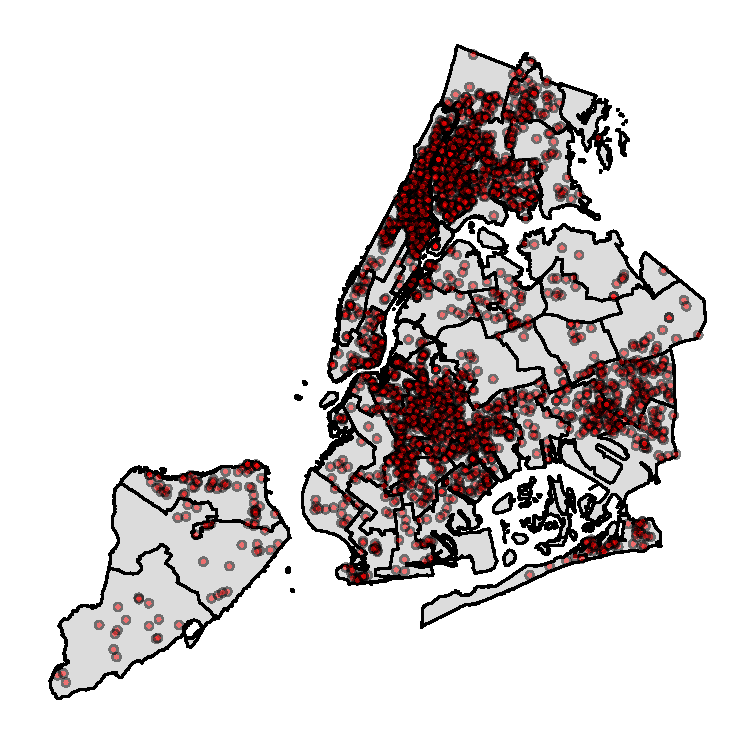
\includegraphics{p1_files/figure-latex/citywide-map-1} 

}

\caption{\label{fig:citymap}Lost Voters on Election Day, 2017}\label{fig:citywide-map}
\end{figure}

Although 73,223 individuals were formally disenfranchised as of the 2017 election, there were just 6,166 disenfranchised voters statewide who had participated in the past 10 years.\footnote{Because address prior to incarceration is not available for individuals who were not registered to vote, computing the total number of formally disenfranchised individuals in New York City is not possible.} Just 8.4 percent of formally disenfranchised individuals, therefore, were individuals with a demonstrated history of participating.

The spatial concentration of lost voters is readily apparent. In some communities, such as Greenwich Village and Brooklyn Heights, hardly any voters were disqualified from participating in the 2017 elections. In other communities, such as Harlem and Central Brooklyn, large numbers of individuals with a demonstrated history of voting were not allowed to cast a ballot for mayor.

\hypertarget{testing-for-neighborhood-turnout-effects}{%
\section*{Testing for Neighborhood Turnout Effects}\label{testing-for-neighborhood-turnout-effects}}
\addcontentsline{toc}{section}{Testing for Neighborhood Turnout Effects}

Table \ref{tab:nhood-dist} shows the distribution of the number of lost voters by neighborhood. Most neighborhoods lost no voters at all; when a neighborhood was home to lost voters, they generally lost just one resident with a history of voting. More than two-thirds of block groups that lost any voters lost only one voter, while 45 percent of census tracts with a lost voter lost only one.

\begin{table}[H]

\caption{\label{tab:distribution-lost}\label{tab:nhood-dist} Distribution of Lost Voters}
\centering
\fontsize{10}{12}\selectfont
\begin{tabular}[t]{ccc}
\toprule
Number of Lost Voters & Count of Block Groups & Count of Tracts\\
\midrule
0 & 4,272 & 1,008\\
1 & 1,023 & 416\\
2 & 301 & 212\\
3 & 107 & 138\\
4 & 30 & 51\\
5 & 19 & 46\\
6 & 9 & 23\\
7 & 3 & 15\\
8 & 5 & 13\\
9 & 0 & 7\\
10 & 0 & 2\\
11 & 0 & 2\\
12 & 0 & 2\\
14 & 0 & 2\\
\hline
Total & 5,769 & 1,937\\
\bottomrule
\end{tabular}
\end{table}

I begin by testing the effect of lost voters on neighborhood turnout using a matching model. Neighborhoods (defined as census tracts and block groups) are considered treated if they were home to \emph{at least one} lost voter in the 2017 election; they are untreated if no voters were disqualified from the election because of a felony conviction. I use a genetic match to match treated to untreated census tracts and block groups (Sekhon \protect\hyperlink{ref-Sekhon2011}{2011}), using a series of demographic and political indicators. Estimates of racial characteristics, median income, education, age, population, and share noncitizen\footnote{The Census Bureau does not make noncitizen estimates available at the block group level. As such, block groups are assigned their census tract's share noncitizen for matching purposes.} come from the Census Bureau's 5-year American Community Survey estimates. Party affiliation rates come from the geocoded voter file. Registration rate is calculated by dividing the number of registered voters (calculated using the voter file) by the citizen voting age population (CVAP, estimated by the Census Bureau). I include voteshare won by the winning city council representative in 2017 as a proxy for the competitiveness of the local race;\footnote{Where neighborhoods cross council district lines, this measure is the mean competitiveness faced by each voter in the neighborhood} where city council district races were more competitive, I expect that more voters will have turned out. Each treated block group is matched to 30 untreated block groups, and each treated census tract is matched with 10 other tracts. Matching is done with replacement. Tables \ref{tab:blockgroup-table} and \ref{tab:tract-table} present the results of these matches.

\hypertarget{match-output}{%
\subsection*{Match Output}\label{match-output}}
\addcontentsline{toc}{subsection}{Match Output}

\begin{table}[H]

\caption{\label{tab:block-table-chunk}\label{tab:blockgroup-table} Results of Block Group-Level Matching}
\centering
\resizebox{\linewidth}{!}{
\begin{tabular}[t]{lllllrrrr}
\toprule
\multicolumn{1}{c}{ } & \multicolumn{2}{c}{Means: Unmatched Data} & \multicolumn{2}{c}{Means: Matched Data} & \multicolumn{4}{c}{Percent Improvement} \\
\cmidrule(l{3pt}r{3pt}){2-3} \cmidrule(l{3pt}r{3pt}){4-5} \cmidrule(l{3pt}r{3pt}){6-9}
 & Treated & Control & Treated & Control & Mean Diff & eQQ Med & eQQ Mean & eQQ Max\\
\midrule
\% Latino & 0.35 & 0.25 & 0.35 & 0.34 & 93.02 & 89.13 & 85.79 & 79.01\\
\% Non-Hispanic Black & 0.38 & 0.16 & 0.38 & 0.37 & 97.93 & 94.46 & 94.41 & 92.77\\
\% Non-Hispanic White & 0.17 & 0.40 & 0.17 & 0.18 & 96.37 & 96.06 & 95.56 & 92.99\\
Median Income & 51,792.52 & 72,612.36 & 51,792.52 & 52,768.97 & 95.31 & 93.47 & 88.62 & 74.49\\
\% With Some College & 0.64 & 0.70 & 0.64 & 0.64 & 90.75 & 94.14 & 90.29 & 80.70\\
Median Age & 35.99 & 38.34 & 35.99 & 36.25 & 89.18 & 90.84 & 85.93 & 78.56\\
Registration Rate & 1.00 & 0.94 & 1.00 & 0.98 & 59.77 & 79.89 & 72.28 & 60.42\\
\% Democrats & 0.75 & 0.65 & 0.75 & 0.75 & 96.22 & 96.52 & 94.92 & 91.02\\
\% Noncitizen & 0.16 & 0.16 & 0.16 & 0.16 & 16.58 & 14.80 & -0.06 & -60.28\\
\% Won by City Council Representative & 0.85 & 0.81 & 0.85 & 0.86 & 89.44 & 83.40 & 79.88 & 70.11\\
\bottomrule
\end{tabular}}
\end{table}

\begin{table}[H]

\caption{\label{tab:tract-table-chunk}\label{tab:tract-table} Results of Tract-Level Matching}
\centering
\resizebox{\linewidth}{!}{
\begin{tabular}[t]{lllllrrrr}
\toprule
\multicolumn{1}{c}{ } & \multicolumn{2}{c}{Means: Unmatched Data} & \multicolumn{2}{c}{Means: Matched Data} & \multicolumn{4}{c}{Percent Improvement} \\
\cmidrule(l{3pt}r{3pt}){2-3} \cmidrule(l{3pt}r{3pt}){4-5} \cmidrule(l{3pt}r{3pt}){6-9}
 & Treated & Control & Treated & Control & Mean Diff & eQQ Med & eQQ Mean & eQQ Max\\
\midrule
\% Latino & 0.32 & 0.22 & 0.32 & 0.33 & 98.55 & 85.12 & 82.84 & 73.01\\
\% Non-Hispanic Black & 0.36 & 0.14 & 0.36 & 0.36 & 99.77 & 88.74 & 88.36 & 83.30\\
\% Non-Hispanic White & 0.19 & 0.42 & 0.19 & 0.19 & 97.50 & 96.32 & 91.29 & 79.95\\
Median Income & 53,409.42 & 71,754.50 & 53,409.42 & 55,422.41 & 89.03 & 90.83 & 84.86 & 62.84\\
\% With Some College & 0.65 & 0.71 & 0.65 & 0.65 & 90.19 & 93.52 & 88.89 & 73.01\\
Median Age & 35.76 & 38.04 & 35.76 & 35.80 & 98.12 & 74.51 & 80.56 & 71.91\\
Registration Rate & 0.94 & 0.90 & 0.94 & 0.93 & 76.63 & 86.16 & 84.24 & 71.28\\
\% Democrats & 0.74 & 0.62 & 0.74 & 0.73 & 94.58 & 94.93 & 92.05 & 82.37\\
\% Noncitizen & 0.16 & 0.17 & 0.16 & 0.17 & -123.57 & 22.48 & 8.85 & -38.79\\
\% Won by City Council Representative & 0.85 & 0.79 & 0.85 & 0.85 & 93.03 & 81.57 & 79.27 & 67.47\\
\bottomrule
\end{tabular}}
\end{table}

At both the tract and block group level, matching results in an untreated group of neighborhoods that looks substantially like the treatment group.

In addition to demonstrating the quality of the genetic match, these tables detail the striking extent to which neighborhoods with lost voters differ from the rest of the city. On average, the non-Hispanic Black share of a block group with a lost voter is more than \emph{double} the share in block groups without lost voters. These impacted neighborhoods are also less than half as non-Hispanic white as unaffected neighborhoods.\footnote{Throughout the remainder of this project, I use White and non-Hispanic White interchangeably. Similarly, Black and non-Hispanic Black are used interchangeably, while Latino indicates Latinos of any race.} The median income in neighborhoods without lost voters is more than 40 percent higher. Tables \ref{tab:blockgroup-table} and \ref{tab:tract-table} throw into sharp relief the types of neighborhoods where likely would-be voters are being disenfranchised due to incarceration and parole.

After matching neighborhoods, I use a simple regression to test whether neighborhood treatment status was associated with turnout in the 2017 mayoral election. Census tract and block group level turnout rates are calculated using the geocoded voter file. Each voter's record indicates whether the voter participated in the 2017 general election, which are then aggregated to estimate the number of ballots cast in each neighborhood. The number of ballots cast is divided by the neighborhood's CVAP.

Much of the literature has discussed whether felony disenfranchisement is particularly demobilizing for eligible Black voters. I therefore include models which explore any potential difference in treatment effect in neighborhoods where a higher share of the population is Black. Table \ref{tab:match-reg} presents the results of these regression models. Robust standard errors are clustered at the level of the match (Abadie and Spiess \protect\hyperlink{ref-Abadie2019}{2019}).

\input{"../../temp/table1.tex"}

When neighborhoods are measured at the block group level, a lost voter is negatively associated with turnout in the 2017 election. In block groups with lost voters, turnout was on average 0.9 percentage points lower than in comparable block groups without lost voters. This decrease, however, appears to be entirely concentrated within Black neighborhoods. When the treatment indicator is interacted with the share of the neighborhood that is non-Hispanic Black, the basic treatment dummy becomes nonsignificant. The coefficient on the interaction between treatment and share Black indicates that treated neighborhoods that are largely Black saw turnout that was as much as 2.7 percentage points lower than similar neighborhoods without lost voters. Considering that the overall turnout rate in block groups with a lost voter was just 14.6 percent, this effect is alarmingly high. For every 100 votes cast in an entirely Black block group with a lost voter, as many as 18.5 votes went uncast. The effects are slightly larger when neighborhoods are measured as block groups than as census tracts, though turnout is still significantly depressed in tracts with lost voters. This is not surprising --- because the spillover effects are likely to operate through social networks, smaller geographical units are likely to be more affected.

\hypertarget{testing-intensity-effects}{%
\subsection*{Testing Intensity Effects}\label{testing-intensity-effects}}
\addcontentsline{toc}{subsection}{Testing Intensity Effects}

Matching methodologies, of course, only allow us to test the effect of being treated --- here, losing any voter for the 2017 election. The models above do not allow for different effects on turnout based on \emph{how many} voters a neighborhood lost, potentially understating the impact of felony disenfranchisement in the most hard-hit communities. In Table \ref{tab:trad-reg} below, I adopt a standard ordinary least squares regression to investigate whether lost voters are associated with lower turnout rates in the 2017 election. This regression uses the same covariates used in the matching procedure described above. Robust standard errors are clustered by city council district.\footnote{Where neighborhoods cross city council district lines, they are assigned the district in which most of their voters live for clustering purposes.}

\input{"../../temp/table2.tex"}

The results presented in Table \ref{tab:trad-reg} align closely with the estimated effect from the matching model. Lost voters are generally associated with lower turnout (each missing voter in a block group reduces that neighborhood's turnout by about 0.82 percentage points), but Models 2 and 4 again make clear that this effect is concentrated in Black neighborhoods. In neighborhoods where most residents are Black, each lost voter is associated with a turnout decrease of up to 1.87 percentage points. The neighborhoods most affected by felony disenfranchisement are neighborhoods where incarceration patterns overlap with Black communities.

The block groups where these depressive effects are concentrated are not randomly distributed throughout the city. They are highly spatially concentrated in Central Brooklyn, Eastern Queens, and Harlem. Figure \ref{fig:postest} applies the coefficient on \(Lost\ Voters \times Share\ Black\) from Model 2 in Table \ref{tab:trad-reg} to the city's block groups. The estimated depressive effect is \(-0.019\times Lost\ Voters \times Share\ Black\).

\begin{figure}[H]

{\centering 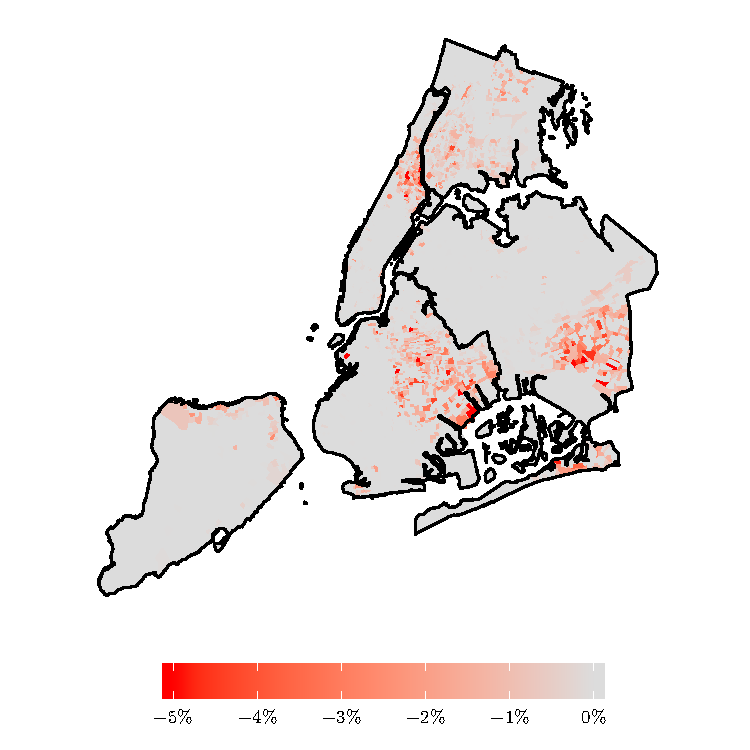
\includegraphics{p1_files/figure-latex/postest-map-1} 

}

\caption{\label{fig:postest}Estimated Depressive Effect of Felony Disenfranchisement}\label{fig:postest-map}
\end{figure}

\hypertarget{toward-a-causal-estimation}{%
\subsection*{Toward a Causal Estimation}\label{toward-a-causal-estimation}}
\addcontentsline{toc}{subsection}{Toward a Causal Estimation}

As the analyses above make clear, neighborhoods with lost voters saw substantially lower turnout in the 2017 mayoral election than neighborhoods without lost voters. The possibility remains, however, that treated neighborhoods systematically differ from untreated neighborhoods in ways that cannot be accounted for using the available data. If that were the case, we would expect that these treated neighborhoods would have lower turnout regardless of whether they lost a voter. As the analysis that follows shows, this is not the case: prior to losing a voter, treated neighborhoods did not have systematically lower turnout than other neighborhoods.

I begin by restricting the set of neighborhoods to only neighborhoods that, on election day in 2016, had no lost voters. This process is the inverse of the process described above: I identify all individuals who were in prison or on parole on November 8\textsuperscript{th}, 2016, who had cast a ballot between 2006 and 2015. These individuals' home neighborhoods are removed from the subsequent analysis. I then use the genetic match algorithm discussed above to match neighborhoods with a lost voter in 2017 to neighborhoods with no lost voters in 2017. These neighborhoods, therefore, were \emph{newly} home to lost voters. If lost voters have no effect on neighborhood turnout, we would expect these treated neighborhoods to have lower turnout in both 2016 --- before they lost a voter --- and in 2017, after a voter was disenfranchised. In 2017, 1,497 neighborhoods had a lost voter; of these, 326 had no lost voters in 2016 and are included here. The original set of control block groups included 4,272 neighborhoods with no lost voters; of these, 211 \emph{did} have a lost voter in 2016, and are thus excluded from this analysis.

Of course, felony disenfranchisement could structure neighborhood turnout differently for presidential and local elections. It is conceivable that the incarceration of a family member or neighbor would sour individuals on participating in local contests, but that the same individual would not read national politics through the same lens. Nevertheless, data limitations makes the 2016 election the only reasonable comparator for 2017 turnout.

Tables \ref{tab:did-match} and \ref{tab:did-match-tract} present the results of matching on these subsets of neighborhoods. As before, the match results in a highly balanced panel between treated and untreated neighborhoods.

\begin{table}[H]

\caption{\label{tab:block-table-chunk-did}\label{tab:did-match} Results of Block Group-Level Matching}
\centering
\resizebox{\linewidth}{!}{
\fontsize{10}{12}\selectfont
\begin{tabular}[t]{lllllrrrr}
\toprule
\multicolumn{1}{c}{ } & \multicolumn{2}{c}{Means: Unmatched Data} & \multicolumn{2}{c}{Means: Matched Data} & \multicolumn{4}{c}{Percent Improvement} \\
\cmidrule(l{3pt}r{3pt}){2-3} \cmidrule(l{3pt}r{3pt}){4-5} \cmidrule(l{3pt}r{3pt}){6-9}
 & Treated & Control & Treated & Control & Mean Diff & eQQ Med & eQQ Mean & eQQ Max\\
\midrule
\% Latino & 0.35 & 0.25 & 0.35 & 0.35 & 99.00 & 96.26 & 94.92 & 85.60\\
\% Non-Hispanic Black & 0.33 & 0.16 & 0.33 & 0.33 & 99.02 & 96.57 & 95.67 & 90.10\\
\% Non-Hispanic White & 0.21 & 0.41 & 0.21 & 0.21 & 99.61 & 94.66 & 92.61 & 82.94\\
Median Income & 55,852.62 & 73,433.49 & 55,852.62 & 56,287.76 & 97.52 & 87.85 & 86.56 & 72.89\\
\% With Some College & 0.65 & 0.71 & 0.65 & 0.65 & 99.31 & 92.25 & 87.30 & 71.15\\
Median Age & 36.17 & 38.47 & 36.17 & 36.04 & 94.37 & 62.35 & 72.27 & 69.84\\
Registration Rate & 0.98 & 0.94 & 0.98 & 0.95 & 25.09 & 46.49 & 42.16 & 33.06\\
\% Democrats & 0.73 & 0.64 & 0.73 & 0.73 & 95.94 & 94.99 & 93.62 & 86.68\\
\% Noncitizen & 0.17 & 0.16 & 0.17 & 0.17 & 63.46 & 75.01 & 66.85 & 45.71\\
\% Won by City Council Representative & 0.85 & 0.80 & 0.85 & 0.85 & 88.19 & 83.99 & 78.23 & 67.54\\
\bottomrule
\end{tabular}}
\end{table}

\begin{table}[H]

\caption{\label{tab:tract-chunk-did}\label{tab:did-match-tract} Results of Tract-Level Matching}
\centering
\resizebox{\linewidth}{!}{
\fontsize{10}{12}\selectfont
\begin{tabular}[t]{lllllrrrr}
\toprule
\multicolumn{1}{c}{ } & \multicolumn{2}{c}{Means: Unmatched Data} & \multicolumn{2}{c}{Means: Matched Data} & \multicolumn{4}{c}{Percent Improvement} \\
\cmidrule(l{3pt}r{3pt}){2-3} \cmidrule(l{3pt}r{3pt}){4-5} \cmidrule(l{3pt}r{3pt}){6-9}
 & Treated & Control & Treated & Control & Mean Diff & eQQ Med & eQQ Mean & eQQ Max\\
\midrule
\% Latino & 0.31 & 0.22 & 0.31 & 0.30 & 94.34 & 86.10 & 84.77 & 75.82\\
\% Non-Hispanic Black & 0.25 & 0.12 & 0.25 & 0.25 & 99.28 & 89.75 & 86.62 & 77.90\\
\% Non-Hispanic White & 0.29 & 0.44 & 0.29 & 0.28 & 97.02 & 87.45 & 77.73 & 61.67\\
Median Income & 59,990.43 & 72,565.90 & 59,990.43 & 61,973.89 & 84.23 & 78.35 & 76.98 & 66.57\\
\% With Some College & 0.67 & 0.71 & 0.67 & 0.66 & 96.86 & 86.51 & 83.73 & 76.55\\
Median Age & 36.36 & 38.23 & 36.36 & 36.39 & 98.60 & 73.15 & 69.00 & 42.11\\
Registration Rate & 0.92 & 0.90 & 0.92 & 0.91 & 10.68 & 64.27 & 63.46 & 56.35\\
\% Democrats & 0.69 & 0.62 & 0.69 & 0.68 & 91.23 & 90.06 & 87.35 & 76.31\\
\% Noncitizen & 0.18 & 0.17 & 0.18 & 0.18 & 78.09 & 73.55 & 62.03 & 48.36\\
\% Won by City Council Representative & 0.83 & 0.79 & 0.83 & 0.83 & 99.91 & 75.59 & 65.98 & 38.91\\
\bottomrule
\end{tabular}}
\end{table}

In Table \ref{tab:did-reg}, I present the outcome of a simple least squares regression on this subset of block groups and tracts. In both models, D(2017) indicates that across the board turnout in 2017 was far lower than in 2016. D(Treat) can be understood as the difference between treated and control neighborhoods in the 2016 election. In Model 1, the treated and control neighborhoods did not have statistically significantly different turnout in the 2016 election; Model 2 indicates that treated census tracts had slightly \emph{higher} turnout prior to intervention. D(Treat) \(\times\) D(2017) is the coefficient of most interest here: it indicates whether, after treatment, treated neighborhoods turned out at lower rates than similar neighborhoods. In Model 1, this coefficient is negative and statistically significant, and is very similar to the coefficients reported in Tables \ref{tab:match-reg} and \ref{tab:trad-reg}. Model 1 in Table \ref{tab:did-reg} indicates that, in the first election after the removal of a voter, a neighborhood's turnout rate decreased by 2.6 percentage points. The relationship does not hold for tracts (suprisingly, treated tracts turned out at higher rates both before and after treatment than control tracts).

\input{"../../temp/table1111.tex"}

Table \ref{tab:did-reg} makes clear that the removal of lost voters likely has a causal effect on neighborhoods' turnout rates. It is worth noting that this is the treatment effect on the treated --- which is to say, it is estimated using only neighborhoods with no lost voters in 2016. These neighborhoods may differ from neighborhoods that had lost voters in both 2016 and 2017. Indeed, neighborhoods that consistently have lost voters are more likely to be the places most impacted by policing patterns. Among block groups that had a lost voter in 2017, those who had no lost voters in 2016 were higher-income (\$51k versus \$56k), had higher shares non-Hispanic White (16 percent versus 21 percent), a lower share non-Hispanic Black (39 percent versus 33 percent), and a smaller share were registered as Democrats (76 percent versus 73 percent).\footnote{Each of these differences are significant at the 99 percent confidence level.} Each of these differences were even more magnified when comparing tracts included in this analysis to all tracts with lost voters in 2017.

Of particular note is the lower share of the population in these neighborhoods that is Black. The analyses above indicate that neighborhoods with more Black residents respond the most strongly to felony disenfranchisement. The set of neighborhoods in this section, therefore, are likely among the least likely to see this relationship. Nevertheless, that this relationship can be detected at the block group level lends credence to the causal relationship between lost voters and depressed turnout.

\hypertarget{discussion}{%
\section*{Discussion}\label{discussion}}
\addcontentsline{toc}{section}{Discussion}

During the 2017 mayoral election, felony disenfranchisement laws were responsible for removing an estimated 2,518 voters from New York City neighborhoods. The spatial concentration of these lost voters is striking, as demonstrated in Figure \ref{fig:citywide-map}, and the systematic removal of voters from these neighborhoods is troubling. However, more than one million votes were cast in the general election of 2017. Although felony disenfranchisement rules have implications for the individuals targeted by them, the removal of such a small number of voters --- concentrated though they are --- is unlikely to have large implications on its own.

As this analysis makes clear, however, felony disenfranchisement reaches beyond the individuals who are incarcerated. Previous literature has established that felony disenfranchisement impacts Black turnout at the state level, but this analysis demonstrates that these demobilizing effects intersect with geographical space to systematically depress the vote in neighborhoods where voters are being sent to prison. As discussed above, these neighborhoods have far lower incomes than the rest of the city: the median income of block groups without any lost voters is more than 40 percent higher than the median income of block groups with lost voters. Similarly, just 17 percent of individuals in the average block group with a lost voter were White, compared with 40 percent of the population in other block groups. Felony disenfranchisement has spillover effects on neighborhood turnout, and these neighborhoods systematically differ from the rest of the city's population. The effects are concentrated in neighborhoods where the most marginalized members of society live. These highly concentrated spillover effects are cause for major concern.

Of equal concern is the apparent concentration of these effects in Black neighborhoods. Both Tables \ref{tab:match-reg} and \ref{tab:trad-reg} indicate that once the lost voter indicator is interacted with the share of a neighborhood that is non-Hispanic Black, the lost voter indicator is either nonsignificant or significant and positive. This means that lost voters have no spillover effects in neighborhoods with small Black populations. Understanding the magnitude of this finding is important. In New York City, there are 1386 block groups where the Black community makes up more than 38 percent of the population (the average for treated block groups), with an average of 912 voting age citizens. Model 2 of Table \ref{tab:match-reg} indicates that, in a block group that is 38 percent Black with a citizen voting age population of 912, having any lost voter reduced turnout by 9.4 ballots. Conversely, in a block group with the same voting age population that is just 16 percent Black (the average for untreated block groups), the loss of any voter decreased turnout by just 3.8 ballots.

The standard OLS regression results tell a similar story: in our average block group that is 38 percent Black, each lost voter cost the neighborhood 6.5 ballots. In block groups of the same size where the population is just 16 percent Black, lost voters cost the neighborhood just 1.6 ballots --- hardly more votes than the lost voter herself.

Why do lost voters in Black neighborhoods have such large spillover effects, when lost voters in predominantly non-Black neighborhoods do not? Much of the previous literature in this space establishes that individuals who have negative interactions with the government are less likely to choose to interact with the state in the future --- that these interactions have large ``interpretive effects'' (Pierson \protect\hyperlink{ref-Pierson1993}{1993}). Lerman and Weaver (\protect\hyperlink{ref-Lerman2013}{2013}), for instance, shows that neighborhoods where there are many police stops that involve searches or use of force use 311 services less frequently. Weaver and Lerman (\protect\hyperlink{ref-Weaver2010}{2010}) argues that interactions with the criminal justice system changes how individuals understand both their identities as citizens and the nature of governmental structures. Similarly, Weaver and Lerman (\protect\hyperlink{ref-Weaver2014}{2014}) tells us that those who have had contact with the criminal justice system consider political participation not just unfruitful but rather ``as something to be actively avoided'' (16). It is perhaps unsurprising that the negative spillover effects are largest in neighborhoods where police presence and criminal justice involvement is most keenly (and unfairly) felt; namely, in plurality and majority Black neighborhoods.

Individuals who live in neighborhoods where police activity is relatively limited may interpret the incarceration of a neighbor as a largely individual phenomenon. If it is understood as an isolated or individual event, voters in these neighborhoods who are not incarcerated are not likely to update their view of the state. They may draw no connections between their neighbor's imprisonment and their own efficacy as a voter. In the neighborhoods where policing is most prevalent --- often, lower-income Black communities --- the incarceration of a neighbor might not be interpreted so individualistically. It may, rather, be interpreted as another reminder of the government's unfairness. If a would-be voter finds herself soured on political participation because of her neighbor's incarceration, she may be less likely to cast a ballot.

This finding mirrors White (\protect\hyperlink{ref-White2019}{2019}\protect\hyperlink{ref-White2019}{a}), which finds that brief jail spells decrease future participation more for Black individuals than for White individuals. This is perhaps unsurprising. A large body of research indicates that, even after controlling for various sociodemographic characteristics and interactions with the police, Black Americans have far more negative views of the criminal justice system than White Americans (e.g.~Browning and Cao \protect\hyperlink{ref-Browning1992}{1992}; Hurwitz and Peffley \protect\hyperlink{ref-Hurwitz2005}{2005}; Henderson et al. \protect\hyperlink{ref-Henderson1997}{1997}; Wu, Sun, and Triplett \protect\hyperlink{ref-Wu2009}{2009}). Experience with the criminal justice system is less likely to be viewed in isolation (and therefore more likely to affect voting patterns) in Black neighborhoods. There is therefore strong reason to suspect that the concentrated depressive effects of felony disenfranchisement in Black neighborhoods arise from these distinct interpretations of the act of incarceration by the state.

For decades, scholars have detailed the problems associated with poor and segregated urban neighborhoods (Wilson \protect\hyperlink{ref-Wilson1990}{1990}). More recent work has begun to interrogate the ways in which the increasing reach of the carceral state shapes the economic and political behavior of individuals caught up in the criminal justice system and their community members. Much of this work, however, has focused on either the impacts of living in marginalized communities (by measuring health and economic impacts) or has not accounted for the importance of physical space (by focusing only on proximal social, and not geographic, contact with directly impacted individuals). This analysis allows us to understand the implications for living in a neighborhood where individuals likely to cast a ballot are not allowed to because of a felony conviction. I find that neighborhoods that are home to lost voters --- and particularly neighborhoods with large Black populations --- systematically turn out for local elections at lower rates than otherwise similar neighborhoods.

This has major ramifications for how we understand the political positioning of the minority neighborhoods most impacted by overpolicing and incarceration. In the case of the 2017 election, there were likely no electoral consequences: Bill de Blasio won reelection handily, and neighborhoods with lost voters overwhelmingly supported his candidacy. A lack of electoral consequences in 2017, however, should not be interpreted to mean that the disparate and concentrated depressive effects of felony disenfranchisement never have implications for who is elected to local office. As Hajnal and Trounstine (\protect\hyperlink{ref-Hajnal2005}{2005}) shows, racial turnout differentials can have real consequences for city politics.

Moreover, we cannot conclude that depressed turnout in these neighborhoods in 2017 had no impact on their representation. City council members representing these neighborhoods, for instance, may determine that pushing for policies popular with these constituents (such as stricter police oversight) will not garner enough votes to make such a fight worthwhile. Although spillover effects from felony disenfranchisement may not have changed who won power in 2017, it very possibly altered how those individuals \emph{held} and \emph{used} their power.

Felony disenfranchisement laws, originally adopted during Jim Crow, have taken on a new life in the era of mass incarceration. Abundant research has demonstrated the pernicious ways in which overincarceration dogs the lives of poor and non-White Americans. As this study shows, however, the neighborhoods bearing the brunt of felony disenfranchisement are also seeing their political power diminished through reduced turnout. The interlocking nature of racioeconomic segregation, politicing patterns, and felony disenfranchisement all combine to undermine the political power of marginalized communities in New York City.

\newpage

\hypertarget{references}{%
\section*{References}\label{references}}
\addcontentsline{toc}{section}{References}

\setlength{\parindent}{-0.5in}
\setlength{\leftskip}{0.5in}

\noindent

\hypertarget{refs}{}
\leavevmode\hypertarget{ref-Abadie2019}{}%
Abadie, Alberto, and Jann Spiess. 2019. ``Robust Post-Matching Inference.'' \url{https://scholar.harvard.edu/spiess/publications/robust-post-matching-inference.}

\leavevmode\hypertarget{ref-Alexander2012}{}%
Alexander, Michelle. 2012. \emph{The New Jim Crow}. New York: The New Press.

\leavevmode\hypertarget{ref-Anzia2019}{}%
Anzia, Sarah F. 2019. ``When Does a Group of Citizens Influence Policy? Evidence from Senior Citizen Participation in City Politics.'' \emph{The Journal of Politics} 81 (1): 1--14. \url{https://doi.org/10.1086/699916}.

\leavevmode\hypertarget{ref-Bowers2009}{}%
Bowers, Melanie, and Robert R. Preuhs. 2009. ``Collateral Consequences of a Collateral Penalty: The Negative Effect of Felon Disenfranchisement Laws on the Political Participation of Nonfelons.'' \emph{Social Science Quarterly} 90 (3): 722--43. \url{https://doi.org/10.1111/j.1540-6237.2009.00640.x}.

\leavevmode\hypertarget{ref-bcj_laws}{}%
Brennan Center for Justice. 2018. ``Criminal Disenfranchisement Laws Across the United States.'' \url{https://www.brennancenter.org/criminal-disenfranchisement-laws-across-united-states}.

\leavevmode\hypertarget{ref-Browning1992}{}%
Browning, Sandra Lee, and Liqun Cao. 1992. ``The Impact of Race on Criminal Justice Ideology.'' \emph{Justice Quarterly} 9 (4): 685--701. \url{https://doi.org/10.1080/07418829200091611}.

\leavevmode\hypertarget{ref-Burch2011}{}%
Burch, Traci. 2011. ``Turnout and Party Registration Among Criminal Offenders in the 2008 General Election.'' \emph{Law and Society Review} 45 (3): 699--730. \url{https://doi.org/10.1111/j.1540-5893.2011.00448.x}.

\leavevmode\hypertarget{ref-Burch2013}{}%
---------. 2013. ``Effects of Imprisonment and Community Supervision on Neighborhood Political Participation in North Carolina.'' Edited by Christopher Wildeman, Jacob S. Hacker, and Vesla M. Weaver. \emph{The ANNALS of the American Academy of Political and Social Science} 651 (1): 184--201. \url{https://doi.org/10.1177/0002716213503093}.

\leavevmode\hypertarget{ref-Cho2006}{}%
Cho, Wendy K. Tam, James G. Gimpel, and Joshua J. Dyck. 2006. ``Residential Concentration, Political Socialization, and Voter Turnout.'' \emph{The Journal of Politics} 68 (1): 156--67. \url{https://doi.org/10.1111/j.1468-2508.2006.00377.x}.

\leavevmode\hypertarget{ref-Clear2008}{}%
Clear, Todd R. 2008. ``The Effects of High Imprisonment Rates on Communities.'' \emph{Crime and Justice} 37 (1): 97--132. \url{https://doi.org/10.1086/522360}.

\leavevmode\hypertarget{ref-Dawkins2006}{}%
Dawkins, Casey J. 2006. ``Are Social Networks the Ties That Bind Families to Neighborhoods?'' \emph{Housing Studies} 21 (6): 867--81. \url{https://doi.org/10.1080/02673030600917776}.

\leavevmode\hypertarget{ref-Drucker2005}{}%
Drucker, Ernest, and Ricardo Barreras. 2005. ``Studies of Voting Behavior and Felony Disenfranchisement Among Individuals in the Criminal Justice System in New York, Connecticut, and Ohio.'' Research report. Sentencing Project. \url{https://www.prisonpolicy.org/scans/sp/fd_studiesvotingbehavior.pdf}.

\leavevmode\hypertarget{ref-Foladare1968}{}%
Foladare, Irving S. 1968. ``The Effect of Neighborhood on Voting Behavior.'' \emph{Political Science Quarterly} 83 (4): 516. \url{https://doi.org/10.2307/2146812}.

\leavevmode\hypertarget{ref-Geller2014}{}%
Geller, Amanda, Jeffrey Fagan, Tom Tyler, and Bruce G. Link. 2014. ``Aggressive Policing and the Mental Health of Young Urban Men.'' \emph{American Journal of Public Health} 104 (12): 2321--7. \url{https://doi.org/10.2105/ajph.2014.302046}.

\leavevmode\hypertarget{ref-Gelman2007}{}%
Gelman, Andrew, Jeffrey Fagan, and Alex Kiss. 2007. ``An Analysis of the New York City Police Departments ``Stop-and-Frisk'' Policy in the Context of Claims of Racial Bias.'' \emph{Journal of the American Statistical Association} 102 (479): 813--23. \url{https://doi.org/10.1198/016214506000001040}.

\leavevmode\hypertarget{ref-Gerber2003}{}%
Gerber, Alan S., Donald P. Green, and Ron Shachar. 2003. ``Voting May Be Habit-Forming: Evidence from a Randomized Field Experiment.'' \emph{American Journal of Political Science} 47 (3): 540--50. \url{https://doi.org/10.1111/1540-5907.00038}.

\leavevmode\hypertarget{ref-Gerber2014}{}%
Gerber, Alan S., Gregory A. Huber, Marc Meredith, Daniel R. Biggers, and David J. Hendry. 2014. ``Can Incarcerated Felons Be (Re)integrated into the Political System? Results from a Field Experiment.'' \emph{American Journal of Political Science} 59 (4): 912--26. \url{https://doi.org/10.1111/ajps.12166}.

\leavevmode\hypertarget{ref-Gerber2017}{}%
---------. 2017. ``Does Incarceration Reduce Voting? Evidence About the Political Consequences of Spending Time in Prison.'' \emph{The Journal of Politics} 79 (4): 1130--46. \url{https://doi.org/10.1086/692670}.

\leavevmode\hypertarget{ref-Gimpel2004}{}%
Gimpel, James G., Joshua J. Dyck, and Daron R. Shaw. 2004. ``Registrants, Voters, and Turnout Variability Across Neighborhoods.'' \emph{Political Behavior} 26 (4): 343--75. \url{https://doi.org/10.1007/s11109-004-0900-4}.

\leavevmode\hypertarget{ref-Griffin2005}{}%
Griffin, John D., and Brian Newman. 2005. ``Are Voters Better Represented?'' \emph{The Journal of Politics} 67 (4): 1206--27. \url{https://doi.org/10.1111/j.1468-2508.2005.00357.x}.

\leavevmode\hypertarget{ref-Guest1999}{}%
Guest, Avery M., and Susan K. Wierzbicki. 1999. ``Social Ties at the Neighborhood Level.'' \emph{Urban Affairs Review} 35 (1): 92--111. \url{https://doi.org/10.1177/10780879922184301}.

\leavevmode\hypertarget{ref-Hajnal2009}{}%
Hajnal, Zoltan. 2009. \emph{America's Uneven Democracy}. Cambridge University Press. \url{https://doi.org/10.1017/cbo9780511800535}.

\leavevmode\hypertarget{ref-Hajnal2005}{}%
Hajnal, Zoltan, and Jessica Trounstine. 2005. ``Where Turnout Matters: The Consequences of Uneven Turnout in City Politics.'' \emph{The Journal of Politics} 67 (2): 515--35. \url{https://doi.org/10.1111/j.1468-2508.2005.00327.x}.

\leavevmode\hypertarget{ref-Henderson1997}{}%
Henderson, Martha L., Francis T. Cullen, Liqun Cao, Sandra Lee Browning, and Renee Kopache. 1997. ``The Impact of Race on Perceptions of Criminal Injustice.'' \emph{Journal of Criminal Justice} 25 (6): 447--62. \url{https://doi.org/10.1016/s0047-2352(97)00032-9}.

\leavevmode\hypertarget{ref-Huckfeldt1979}{}%
Huckfeldt, R. Robert. 1979. ``Political Participation and the Neighborhood Social Context.'' \emph{American Journal of Political Science} 23 (3): 579. \url{https://doi.org/10.2307/2111030}.

\leavevmode\hypertarget{ref-Hurwitz2005}{}%
Hurwitz, Jon, and Mark Peffley. 2005. ``Explaining the Great Racial Divide: Perceptions of Fairness in the U.s. Criminal Justice System.'' \emph{The Journal of Politics} 67 (3): 762--83. \url{https://doi.org/10.1111/j.1468-2508.2005.00338.x}.

\leavevmode\hypertarget{ref-Kenny1992}{}%
Kenny, Christopher B. 1992. ``Political Participation and Effects from the Social Environment.'' \emph{American Journal of Political Science} 36 (1): 259. \url{https://doi.org/10.2307/2111432}.

\leavevmode\hypertarget{ref-Keyssar2009}{}%
Keyssar, Alexander. 2009. \emph{The Right to Vote: The Contested History of Democracy in the United States}. New York: Basic Books.

\leavevmode\hypertarget{ref-King2016}{}%
King, Bridgett A., and Laura Erickson. 2016. ``Disenfranchising the Enfranchised.'' \emph{Journal of Black Studies} 47 (8): 799--821. \url{https://doi.org/10.1177/0021934716659195}.

\leavevmode\hypertarget{ref-Kinsella2015}{}%
Kinsella, Chad, Colleen McTague, and Kevin N. Raleigh. 2015. ``Unmasking Geographic Polarization and Clustering: A Micro-Scalar Analysis of Partisan Voting Behavior.'' \emph{Applied Geography} 62 (August): 404--19. \url{https://doi.org/10.1016/j.apgeog.2015.04.022}.

\leavevmode\hypertarget{ref-Lerman2013}{}%
Lerman, Amy E., and Vesla Weaver. 2013. ``Staying Out of Sight? Concentrated Policing and Local Political Action.'' Edited by Christopher Wildeman, Jacob S. Hacker, and Vesla M. Weaver. \emph{The ANNALS of the American Academy of Political and Social Science} 651 (1): 202--19. \url{https://doi.org/10.1177/0002716213503085}.

\leavevmode\hypertarget{ref-locked_out}{}%
Manza, Jeff, and Christopher Uggen. 2006. \emph{Locked Out: Felon Disenfranchisement and American Democracy}. New York: Oxford University Press.

\leavevmode\hypertarget{ref-Martin2003}{}%
Martin, Paul S. 2003. ``Votings Rewards: Voter Turnout, Attentive Publics, and Congressional Allocation of Federal Money.'' \emph{American Journal of Political Science} 47 (1): 110--27. \url{https://doi.org/10.1111/1540-5907.00008}.

\leavevmode\hypertarget{ref-Martin2013}{}%
Martin, Paul S., and Michele P. Claibourn. 2013. ``Citizen Participation and Congressional Responsiveness: New Evidence That Participation Matters.'' \emph{Legislative Studies Quarterly} 38 (1): 59--81. \url{https://doi.org/10.1111/lsq.12003}.

\leavevmode\hypertarget{ref-Meredith2013}{}%
Meredith, Marc, and Michael Morse. 2013. ``Do Voting Rights Notification Laws Increase Ex-Felon Turnout?'' Edited by Christopher Wildeman, Jacob S. Hacker, and Vesla M. Weaver. \emph{The ANNALS of the American Academy of Political and Social Science} 651 (1): 220--49. \url{https://doi.org/10.1177/0002716213502931}.

\leavevmode\hypertarget{ref-Miles2004}{}%
Miles, Thomas J. 2004. ``Felon Disenfranchisement and Voter Turnout.'' \emph{The Journal of Legal Studies} 33 (1): 85--129. \url{https://doi.org/10.1086/381290}.

\leavevmode\hypertarget{ref-Mutz2002}{}%
Mutz, Diana C. 2002. ``The Consequences of Cross-Cutting Networks for Political Participation.'' \emph{American Journal of Political Science} 46 (4): 838. \url{https://doi.org/10.2307/3088437}.

\leavevmode\hypertarget{ref-Ochs2006}{}%
Ochs, Holona Leanne. 2006. ``'Colorblind' Policy in Black and White: Racial Consequences of Disenfranchisement Policy.'' \emph{Policy Studies Journal} 34 (1): 81--93. \url{https://doi.org/10.1111/j.1541-0072.2006.00146.x}.

\leavevmode\hypertarget{ref-Pierson1993}{}%
Pierson, Paul. 1993. ``When Effect Becomes Cause: Policy Feedback and Political Change.'' \emph{World Politics} 45 (4): 595--628. \url{https://doi.org/10.2307/2950710}.

\leavevmode\hypertarget{ref-Sekhon2011}{}%
Sekhon, Jasjeet S. 2011. ``Multivariate and Propensity Score Matching Software with Automated Balance Optimization: The Matching Package for R.'' \emph{Journal of Statistical Software} 42 (7). \url{https://doi.org/10.18637/jss.v042.i07}.

\leavevmode\hypertarget{ref-Sewell2016}{}%
Sewell, Abigail A., and Kevin A. Jefferson. 2016. ``Collateral Damage: The Health Effects of Invasive Police Encounters in New York City.'' \emph{Journal of Urban Health} 93 (S1): 42--67. \url{https://doi.org/10.1007/s11524-015-0016-7}.

\leavevmode\hypertarget{ref-sentencing_2016}{}%
Uggen, Christopher, Ryan Larson, and Sarah Shannon. 2016. ``6 Million Lost Voters: State-Level Estimates of Felony Disenfranchisement, 2016.'' Research report. Sentencing Project. \url{https://www.sentencingproject.org/publications/6-million-lost-voters-state-level-estimates-felony-disenfranchisement-2016/}.

\leavevmode\hypertarget{ref-Uggen2002}{}%
Uggen, Christopher, and Jeff Manza. 2002. ``Democratic Contraction? Political Consequences of Felon Disenfranchisement in the United States.'' \emph{American Sociological Review} 67 (6): 777. \url{https://doi.org/10.2307/3088970}.

\leavevmode\hypertarget{ref-Uggen2004}{}%
---------. 2004. ``Lost Voices: The Civic and Political Views of Disfranchised Felons.'' In \emph{Imprisoning America: The Social Effects of Mass Incarceration}, edited by Mary Pattillo, David Weiman, and Bruce Western, 165--204. New York: Russell Sage Foundation.

\leavevmode\hypertarget{ref-Walker2014}{}%
Walker, Hannah L. 2014. ``Extending the Effects of the Carceral State. Proximal Contact, Political Participation, and Race.'' \emph{Political Research Quarterly} 67 (4): 809--22. \url{https://doi.org/10.1177/1065912914542522}.

\leavevmode\hypertarget{ref-Walker2017}{}%
Walker, Hannah L., and Marcela Garcı́a-Castañon. 2017. ``For Love and Justice: The Mobilizing of Race, Gender, and Criminal Justice Contact.'' \emph{Politics \& Gender} 13 (04): 541--68. \url{https://doi.org/10.1017/s1743923x17000198}.

\leavevmode\hypertarget{ref-Weaver2014}{}%
Weaver, Vesla, and Amy E. Lerman. 2014. \emph{Arresting Citizenship: The Democratic Consequences of American Crime Control}. Chicago: University of Chicago Press.

\leavevmode\hypertarget{ref-Weaver2010}{}%
Weaver, Vesla M., and Amy E. Lerman. 2010. ``Political Consequences of the Carceral State.'' \emph{American Political Science Review} 104 (4): 817--33. \url{https://doi.org/10.1017/s0003055410000456}.

\leavevmode\hypertarget{ref-White2019}{}%
White, Ariel. 2019a. ``Misdemeanor Disenfranchisement? The Demobilizing Effects of Brief Jail Spells on Potential Voters.'' \emph{American Political Science Review} 113 (2): 311--24. \url{https://doi.org/10.1017/s000305541800093x}.

\leavevmode\hypertarget{ref-White2019a}{}%
---------. 2019b. ``Family Matters? Voting Behavior in Households with Criminal Justice Contact.'' \emph{American Political Science Review} 113 (2): 607--13. \url{https://doi.org/10.1017/s0003055418000862}.

\leavevmode\hypertarget{ref-Wilson1990}{}%
Wilson, William Julius. 1990. \emph{The Truly Disadvantaged: The Inner City, the Underclass, and Public Policy}. Chicago: University Of Chicago Press.

\leavevmode\hypertarget{ref-Wu2009}{}%
Wu, Yuning, Ivan Y. Sun, and Ruth A. Triplett. 2009. ``Race, Class or Neighborhood Context: Which Matters More in Measuring Satisfaction with Police?'' \emph{Justice Quarterly} 26 (1): 125--56. \url{https://doi.org/10.1080/07418820802119950}.


\end{document}
